\documentclass[12pt,addpoints]{exam}
\usepackage[utf8]{inputenc}
\usepackage[T1]{fontenc}
\usepackage[brazil]{babel}
\usepackage[a4paper, margin=2cm]{geometry}
\usepackage{graphicx, amsmath, amsfonts, amssymb, xcolor, url, tikz, pgfplots, subfigure}
\usepackage[colorlinks=True,urlcolor=blue]{hyperref}
\newcommand{\disciplina}{Laboratório de Princípios de Comunicações}
\newcommand{\periodo}{2022.1e}
\newcommand{\avaliacao}{Guia de Experimentos 1}
\newcommand{\tema}{Introdução ao GNU Radio. Séries de Fourier. Distorção.}
%\newcommand{\professor}{Bruno\ B.\ Albert e Edmar C.\ Gurjão}
\newcommand{\professor}{Edson P.\ da Silva e Leocarlos B.\ S.\ Lima}
%\newcommand{\professor}{Edson P.\ da Silva e Luciana Veloso}
%\newcommand{\professor}{Edmar C.\ Gurjão e Luciana Veloso}
%\newcommand{\professor}{Bruno\ B.\ Albert e Edson P.\ da Silva}

\pagestyle{head}
\firstpageheader{}{}{}
\runningheader{Lab.\ Princ.\ Comunicações}{\avaliacao}{Página \thepage}
\runningheadrule
\pointpoints{ponto}{pontos}
\newcommand{\myscale}{0.4}

\begin{document}

\noindent \includegraphics[height=2cm]{../Figuras/UFCGLogo.png} \hfill
\begin{minipage}{.66\textwidth} \large \centering \vspace{-1.8cm}
    Universidade Federal de Campina Grande -- UFCG \\
    Unidade Acadêmica de Engenharia Elétrica -- UAEE \\
    Curso de Graduação em Engenharia Elétrica
\end{minipage}
\hfill \includegraphics[height=2cm]{../Figuras/DEELogo.png} \\[12pt]

\noindent
\begin{tabular*}{\textwidth}{lcr}
    \textbf{\disciplina} && \\
    Período \periodo && \\
    \textbf{\avaliacao} && \\
    Tema(s): \tema && \\
    Professor(es): \professor &&
\end{tabular*}
\noindent\rule[2ex]{\textwidth}{2pt}

\section{Introdução}

O presente guia descreve atividades experimentais a serem realizadas na disciplina Laboratório de Princípios de Comunicações do curso de graduação em Engenharia Elétrica da Universidade Federal de Campina Grande -- UFCG.

Os experimentos propostos deverão ser realizados no Laboratório de Princípios de Comunicações -- LPC, localizado na Central de Laboratórios da Unidade Acadêmica de Engenharia Elétrica da UFCG, empregando:
\begin{itemize}
    \item Computador com software GNU Radio Companion -- GRC (\url{http://gnuradio.org/}) instalado;
    \item Módulo USRP (do inglês \textit{Universal Software Radio Peripheral}) para transmissão e recepção de sinais numa abordagem conhecida como Rádio Definido por Software -- RDS.
\end{itemize}

Na seção \ref{sect:Preparacao} deste guia, propõe-se um conjunto de atividades de preparação a serem desenvolvidas pelo aluno antes da aula em que serão realizadas as práticas experimentais. Sem a realização prévia destas atividades pelo aluno, as práticas experimentais propostas ficarão comprometidas, tanto no tempo necessário para sua realização quanto no aproveitamento pelo aluno. Por essa razão, \textbf{o aluno só poderá realizar os experimentos em laboratório se apresentar ao professor no início da aula os resultados da preparação proposta}. 

A aula terá duração de duas horas e o aluno deverá entregar ao seu término, por escrito, respostas às questões referentes aos experimentos realizados propostas na Folha de Respostas (parte final do guia).

\section{Objetivos}

As práticas experimentais aqui propostas têm por objetivos:
\begin{itemize}
    \item Introduzir ao \textit{GNU Radio Companion} como ferramenta para realização de experimentos em comunicações;
    \item Simular e analisar séries de Fourier de sinais comuns;
    \item Caracterizar distorções de canal.
\end{itemize}

\newpage

\section{Preparação} \label{sect:Preparacao}

\subsection{Estudo}

Leia o tutorial introdutório ao uso do GRC, disponível na página \href{http://wiki.gnuradio.org/index.php/Guided_Tutorial_GRC}{Guided Tutorial GRC}, a partir da seção 2.2. Se possível, instale o GRC em seu computador pessoal (veja instruções de instalação em \href{http://wiki.gnuradio.org/index.php/InstallingGR}{InstallingGR}) e experimente os exercícios sugeridos no tutorial.

Revise e pesquise sobre os seguintes questionamentos teóricos\footnote{Sugerimos leitura da seção 3.6 da referência: \begin{quote} LATHI, B. P., DING, Z. \textit{Sistemas de comunicações analógicos e digitais modernos}. 4 ed. [S.l.]: LTC, 2009. \end{quote}}:
\begin{itemize}
    \item O que caracteriza uma distorção linear? 
    \item O que caracteriza uma distorção não linear?
\end{itemize}

Para revisar o conteúdo teórico e responder os problemas da preparação, leia e execute o código do notebook \href{https://github.com/edsonportosilva/LPC/blob/master/Jupyter/Lab1/Lab1.ipynb}{Lab1.ipynb}

\subsection{Problemas}

\begin{questions}
    \question Determine as séries de Fourier trigonométricas das formas de onda periódicas ilustradas na Figura \ref{fig:sinaisusuais}.
    \begin{figure}[htb]
        \centering
        \subfigure[fig:ondaquadrada][Onda quadrada $g_{q}(t)$ de frequência $f = 150$~Hz e amplitude $A = 1$.]{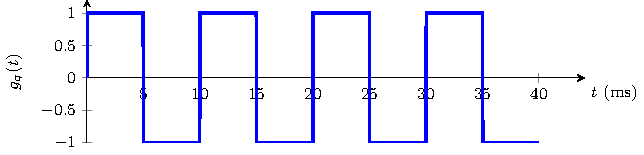
\includegraphics{./Figuras/OndaQuadrada}}\label{subfig:ondaquadrada}
        \qquad
        \subfigure[fig:ondatriangular][Onda triangular $g_{t}(t)$ de frequência $f = 150$~Hz e amplitude $A = 1$.]{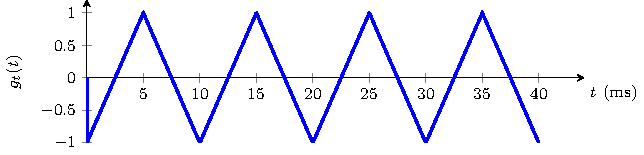
\includegraphics{./Figuras/OndaTriangular}}
        \qquad
        \subfigure[fig:ondadenteserra][Onda dente de serra $g_{d}(t)$ de frequência $f = 150$~Hz e amplitude $A = 1$.]{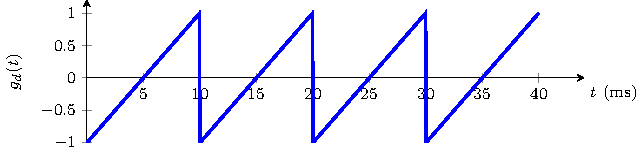
\includegraphics{./Figuras/OndaDenteSerra}}
        \caption{Formas de onda usuais.}
        \label{fig:sinaisusuais}
    \end{figure}

	\question Mudar a frequência fundamental afetará a potência de um sinal periódico? Explique. E a sua ocupação de banda? Explique.
    
    \question A antena do seu aparelho celular capta uma potência de sinal geralmente em torno de $-60$~dBm (excelente conexão) e $-110$~dBm (conexão muito ruim). Quais são os valores de potência em mW correspondentes a estes limiares? E em dBW?
  \end{questions}


\section{Experimentos}

A seguir são descritas práticas experimentais a serem realizadas pelo(a) aluno(a). 

\subsection{Experimento 1 -- GNU Radio Companion}

O objetivo deste experimento é familiarizar o aluno com o GRC e com seus recursos empregados nas práticas experimentais deste laboratório.

\begin{enumerate}
    \item Antes de iniciar as atividades com o GRC, crie uma pasta para guardar os arquivos de seus experimentos e copie nela os modelos de diagrama (arquivos .GRC) disponibilizados pelo professor para esta aula. \textbf{Não deixe de realizar isso, pois o computador deste laboratório não é para seu uso pessoal e os arquivos que você utilizará serão alterados por você durante o experimento};
    \item Execute o software GRC (no Ubuntu, tecle \textbf{Meta $+$ A}, em seguida digite \textbf{grc} e tecle \textbf{Enter}). A janela do GRC deverá aparecer, conforme ilustrado na Figura \ref{fig:GRC_1-1a}.
    \begin{figure}[htb]
        \centering
        \includegraphics[width=\textwidth]{./Figuras/GRC_1-1a} \\
        \caption{Janela do GNU Radio Companion após aberto.} 
        \label{fig:GRC_1-1a}
    \end{figure}
  
    Essa janela possui quatro partes:
    \begin{enumerate}
        \item \textbf{Barra de ferramentas}, parte superior, com botões que permitem desde a abertura de arquivos, até a execução de diagramas;
        \item \textbf{Espaço de trabalho}, parte central, na qual os diagramas são ``desenhados'';
        \item \textbf{Terminal}, parte inferior, na qual são apresentadas informações de execução dos diagramas, mensagens de erro etc.;
        \item \textbf{Biblioteca}, parte direita, na qual são listados todos os blocos funcionais disponíveis no GRC para o projeto de diagramas.
    \end{enumerate}
    \item Clique duas vezes no bloco \textbf{Options} para editar seus parâmetros. Edite-os, conforme a Figura \ref{fig:GRC_1-1b};
    \begin{figure}[htb]
        \centering
        \includegraphics[scale=\myscale]{./Figuras/GRC_1-1b} \\
        \caption{Janela de edição de parâmetros do bloco \textbf{Options}.} 
        \label{fig:GRC_1-1b}
    \end{figure}
    \item De modo similar, edite os parâmetros do bloco \textbf{Variable}, fazendo o campo \textbf{Value} igual a 8000. Esta variável será usada em outros blocos e define a taxa de amostragem adotada em todo o sistema;
    \item Tecle \textbf{Ctrl $+$ F}. Surgirá um campo de busca sobre a Biblioteca do GRC, que permitirá localizar rapidamente blocos. Digite \textbf{Signal Source}. Deverá surgir na Biblioteca um bloco com este nome. Clique duas vezes sobre este item (ou clique no item e o arraste para o Espaço de Trabalho). Isso inserirá um bloco \textbf{Signal Source} no Espaço de Trabalho. Posicione-o, conforme a Figura \ref{fig:GRC_1-1c}.
    \begin{figure}[htb]
        \centering
        \includegraphics[scale=\myscale]{./Figuras/GRC_1-1c} \\
        \caption{Diagrama de blocos, com inclusão do bloco \textbf{Signal Source}.} 
        \label{fig:GRC_1-1c}
    \end{figure}
    \item Edite os parâmetros deste bloco, alterando-os para:
    \begin{itemize}
        \item \textbf{Output Type}: Float;
        \item \textbf{Waveform}: Sine;
        \item \textbf{Frequency}: 125;
        \item \textbf{Amplitude}: 1.0;
    \end{itemize}
    \item De modo similar, introduza no diagrama mais dois blocos: \textbf{Throttle} e \textbf{QT GUI Time Sink}. O primeiro limita o processamento interno do sistema ao número de amostras por segundo definido pela taxa de amostragem, evitando sobrecarregar o processador. Este bloco deve, de modo geral, ser usado em todos os diagramas. O segundo apresenta o gráfico no tempo do sinal aplicado à sua entrada;
    \item Edite os parâmetros de ambos os blocos, fazendo o campo \textbf{Output Type} igual a \textbf{Float}. Edite ainda os seguintes campos do bloco \textbf{QT GUI Time Sink}:
    \begin{itemize}
        \item \textbf{Grid}: Yes;
        \item \textbf{Autoscale}: Yes;
    \end{itemize}
    \item Posicione os blocos no diagrama, conforme a Figura \ref{fig:GRC_1-1d}. Passando o ponteiro do mouse sobre os ``conectores'' dos blocos, pode-se identificar quais são de entrada (in) e quais são de saída (out). Para conectar dois blocos, basta clicar no conector de um bloco e, logo em seguida, no conector do outro bloco. Só podem ser conectados conector de entrada com conector de saída. Uma mesma saída pode ser conectada a mais de uma entrada;
    \begin{figure}[htb]
        \centering
        \includegraphics[scale=\myscale]{./Figuras/GRC_1-1d} \\
        \caption{Diagrama de blocos, com inclusão e interligação dos blocos \textbf{Throttle} e \textbf{QT GUI Time Sink}.} 
        \label{fig:GRC_1-1d}
    \end{figure}
    \item Para executar o diagrama projetado, tecle \textbf{F6}. O gráfico da senoide gerada deverá ser apresentado;
    \item Responda às questões propostas na Folha de Respostas.
\end{enumerate}

\subsection{Experimento 2 -- Séries de Fourier}

Os objetivos deste experimento é produzir uma versão aproximada de um sinal a partir das componentes de sua série trigonométrica de Fourier.

\begin{enumerate}
    \item Execute o software GRC e abra o arquivo \textbf{Labo1-2.grc} disponibilizado pelo professor. A Figura \ref{fig:GRC_1-2} ilustra o diagrama deste experimento. Ele consiste na simples adição de três componentes de frequência (senoides) que, tendo suas amplitudes, fases e frequências corretamente ajustadas em conformidade com uma série de Fourier trigonométrica de um sinal, deve resultar numa aproximação deste sinal;
    \begin{figure}[htb]
        \centering
        \includegraphics[scale=\myscale]{./Figuras/GRC_1-2} \\
        \caption{Diagrama de blocos para geração aproximada de sinais comuns a partir de suas séries trigonométrica de Fourier.} 
        \label{fig:GRC_1-2}
    \end{figure}
    % \item Ajuste frequência, amplitude e fase (seno ou cosseno) destas três senoides de modo a gerar os sinais de onda quadrada $g_{q}(t)$, onda triangular $g_{t}(t)$ e onda dente de serra $g_{d}(t)$, cujas séries de Fourier foram calculadas na etapa de preparação;
    \item Execute o diagrama e responda às questões propostas na Folha de Respostas.
\end{enumerate}

\subsection{Experimento 3 -- Distorção}

O objetivo deste experimento é caracterizar uma distorção de amplitude e de fase sofrida por um sinal.

\begin{enumerate}
    \item Execute o software GRC e abra o arquivo \textbf{Labo1-3.grc} disponibilizado pelo professor. A Figura \ref{fig:GRC_1-3} ilustra o diagrama deste experimento. Ele consiste numa simulação de um canal distorcivo discreto, composto por blocos \textbf{Multiply Const} e \textbf{Delay}, que atenuam e atrasam três componentes individuais de um sinal, permitindo comparar os gráficos temporais dos sinais na entrada e na saída do canal distorcivo;
    \begin{figure}[htb]
        \centering
        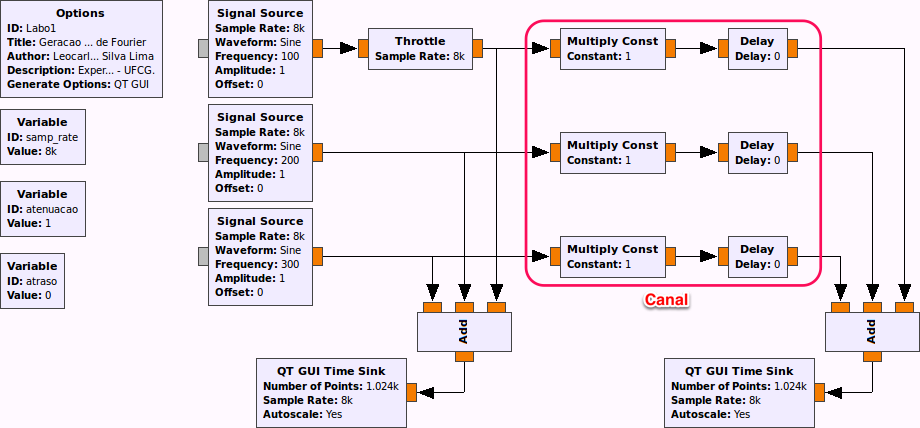
\includegraphics[scale=\myscale]{./Figuras/GRC_1-3} \\
        \caption{Diagrama de blocos para análise do efeito de distorção de amplitude e fase em sinais.} 
        \label{fig:GRC_1-3}
    \end{figure}
    \item Ajuste frequência, amplitude e fase (seno ou cosseno) das três senoides de entrada, de modo a gerar o sinal de onda triangular $g_{t}(t)$, cuja série trigonométrica de Fourier foi calculada na etapa de preparação;    
    \item Execute o diagrama e responda às questões propostas na Folha de Respostas.
\end{enumerate}

\newpage \pagenumbering{arabic}

\noindent \includegraphics[height=2cm]{../Figuras/UFCGLogo} \hfill
\begin{minipage}{.66\textwidth} \large \centering \vspace{-1.8cm}
    Universidade Federal de Campina Grande -- UFCG \\
    Unidade Acadêmica de Engenharia Elétrica -- UAEE \\
    Curso de Graduação em Engenharia Elétrica
\end{minipage}
\hfill \includegraphics[height=2cm]{../Figuras/DEELogo} \\[12pt]

\noindent
\begin{tabular*}{\textwidth}{l @{\extracolsep{\fill}} r @{\extracolsep{6pt}} l}
    \textbf{\disciplina} && \\
    Período \periodo && \\
    \textbf{\avaliacao\ -- Folha de Respostas} && \\
    Tema(s): \tema && \\
    Professor(es): \professor && \\[12pt]
    \textbf{Aluno:} \hrulefill && \textbf{Data:} \makebox[3cm]{\hrulefill}
\end{tabular*}
\noindent\rule[2ex]{\textwidth}{2pt}

\section*{Experimento 1 -- GNU Radio Companion}

\begin{questions}
    \question Por inspeção do gráfico, informe o período da senoide gerada? Você pode aplicar um ``zoom'' no gráfico para melhorar a visualização.
    \fillwithlines{0.25in}

    \question Suponha que desejamos processar um sinal de voz e que o microfone não capta sinais acima de 8 kHz. Qual a taxa de amostragem mínima que devemos colocar no bloco \textbf{Variable:} samp\_rate?
    \fillwithlines{0.25in}
\end{questions}

\section*{Experimento 2 -- Séries de Fourier}

\begin{questions}
    \question Ajuste frequência, amplitude e fase (seno ou cosseno) dessas três senoides conforme as séries de Fourier calculadas na etapa de preparação.
    \begin{parts} 
        \part Para a onda quadrada $g_{q}(t)$, identifique (e informe abaixo) por inspeção no gráfico de tempo a amplitude e o período da forma de onda. Identifique também (e informe abaixo) por inspeção no gráfico de frequências as componentes (frequências e amplitudes em dB) do sinal.
        \fillwithlines{0.5in}
        \part Faça o mesmo para a onda triangular $g_{t}(t)$.
        \fillwithlines{0.5in}
        \part Faça o mesmo para a onda dente de serra $g_{d}(t)$.
        \fillwithlines{0.5in}
    \end{parts}
    
    \question Por que a onda triangular gerada assemelha-se mais à forma de onda original do que às outras duas?
    \fillwithlines{0.5in}

\end{questions}

\section*{Experimento 3 -- Distorção}

\begin{questions}
    \question Observe que os sinais de entrada e saída do canal são idênticos. Esse seria um canal ideal, em que o sinal na entrada é exatamente o mesmo na saída, ou seja o canal não atenua ou atrasa o sinal transmitido.
    \begin{parts}
        \part Na aba {\bf Ganho/Atenuação}, altere os valores de todas as componentes de frequência de 1 para 0.5. Houve distorção? Realize o mesmo procedimento mudando os valores para 1.25. Houve distorção? Descreva o que ocorre com o sinal nestas configurações e dê uma explicação para o que foi observado.
        \fillwithlines{0.5in}
        \part Novamente na aba {\bf Ganho/Atenuação}, retorne os valores da primeira e terceira componentes para 1 e altere o valor da segunda componente para 0.20. Houve distorção? Descreva o que ocorre com o sinal nestas configurações e dê uma explicação para o que foi observado.
        \fillwithlines{0.5in}
        \part Na aba {\bf Ganho/Atenuação}, retorne todos os valores para 1. Na aba {\bf Deslocamento de fase}, altere o valor do deslocamento de fase da primeira componente para 6000. Houve distorção? Descreva o que ocorre com o sinal nestas configurações e dê uma explicação para o que foi observado.
        \fillwithlines{0.5in}
        \part Novamente na aba {\bf Deslocamento de fase}, altere os valores do deslocamento de fase da primeira, segunda e terceira componentes para 2000, 6000 e 10000, respectivamente. Houve distorção? Descreva o que ocorre com o sinal nestas configurações e dê uma explicação para o que foi observado.
        \fillwithlines{0.5in}
        \part É possível identificar distorções de amplitude observando o espectro de potência do sinal? Explique. E distorções de fase?
        \fillwithlines{0.5in} 
         \part As distorções que foram observadas neste experimento são distorções lineares ou não-lineares? Explique.
        \fillwithlines{0.5in}      
    \end{parts}

\end{questions}

\end{document}
